\title{Updated plots for publications}
\author{ }
\date{\today}

\documentclass[12pt]{article}

\usepackage{graphicx,type1cm,eso-pic,color}
\usepackage{mathtools}
\usepackage{feynmp}

\begin{document}

\maketitle

\section*{}


\begin{figure}[tpb]
   \centering
  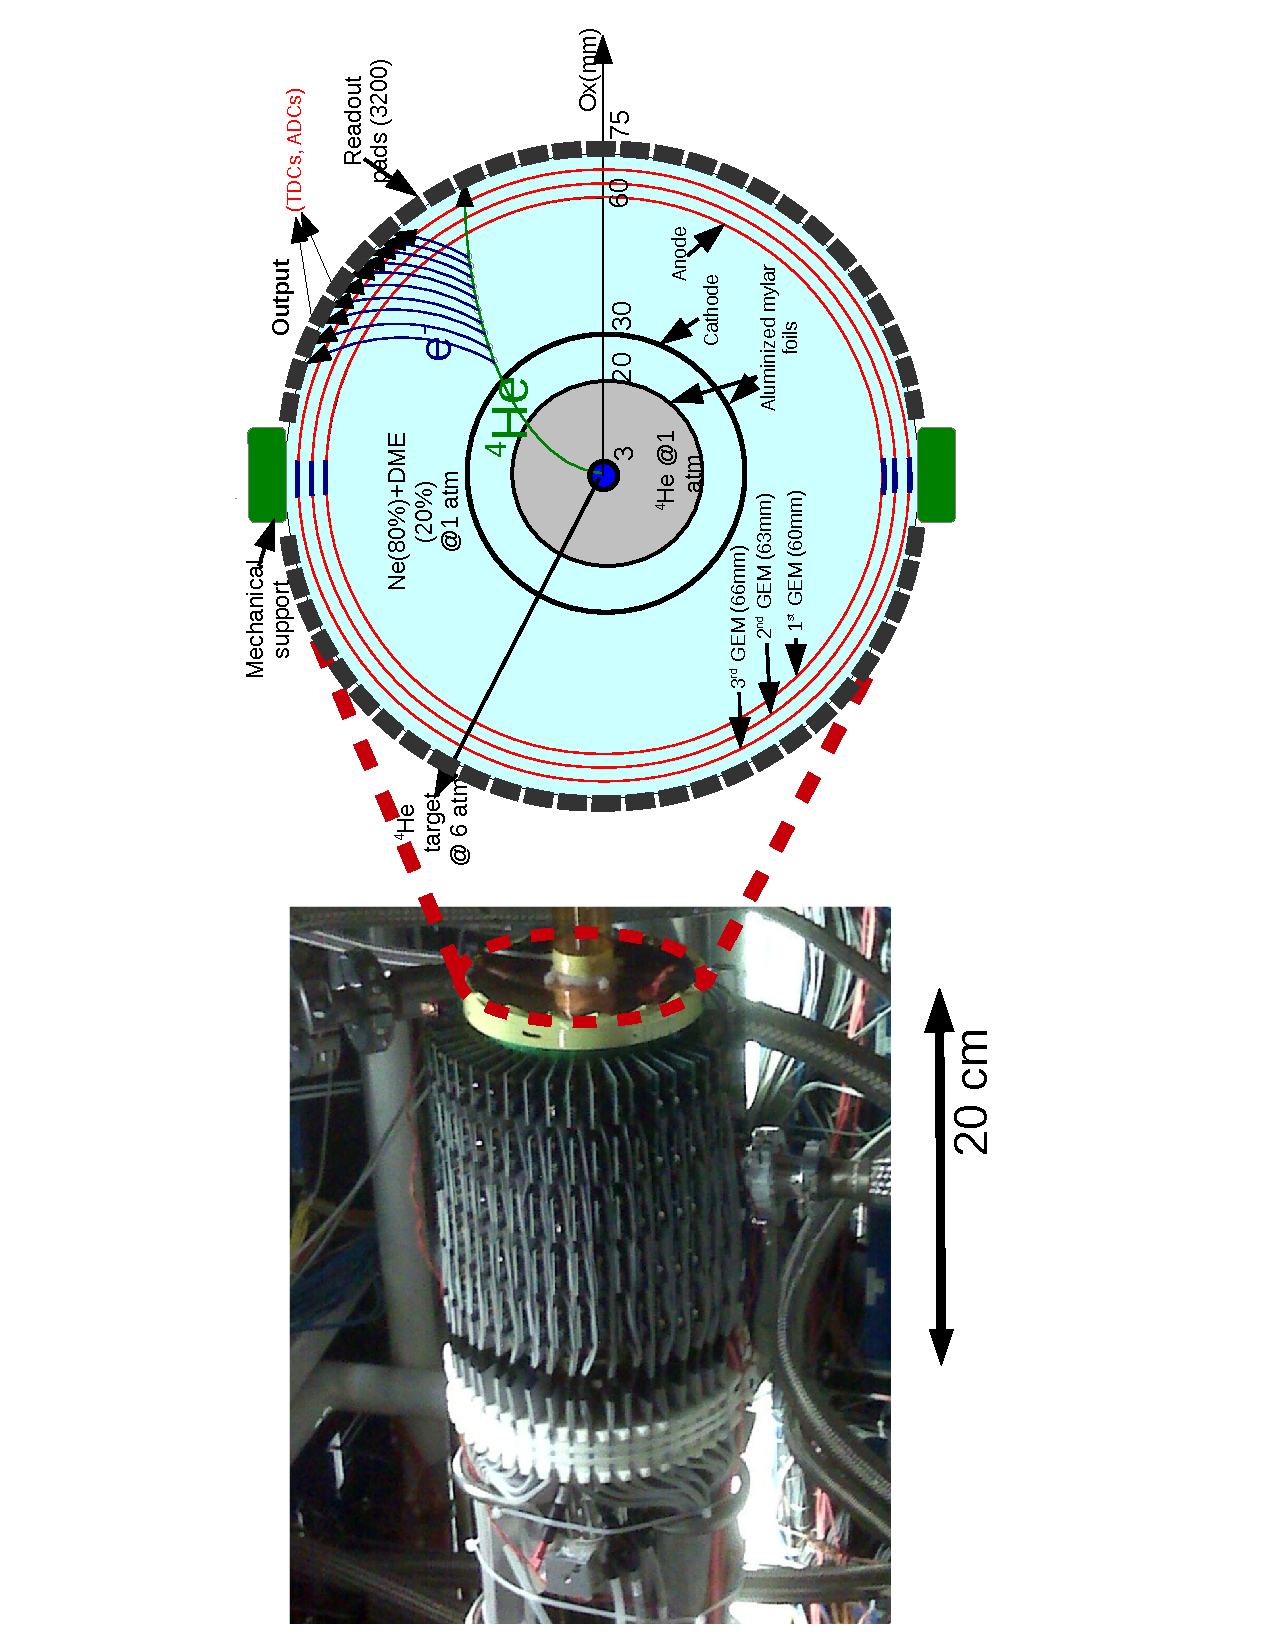
\includegraphics[height=15.0cm, angle =-90]{RTPC.pdf}
  \caption{RTPC.}
  \label{fig:}
 \end{figure}                                                                  


\begin{figure}[tpb]
   \centering
  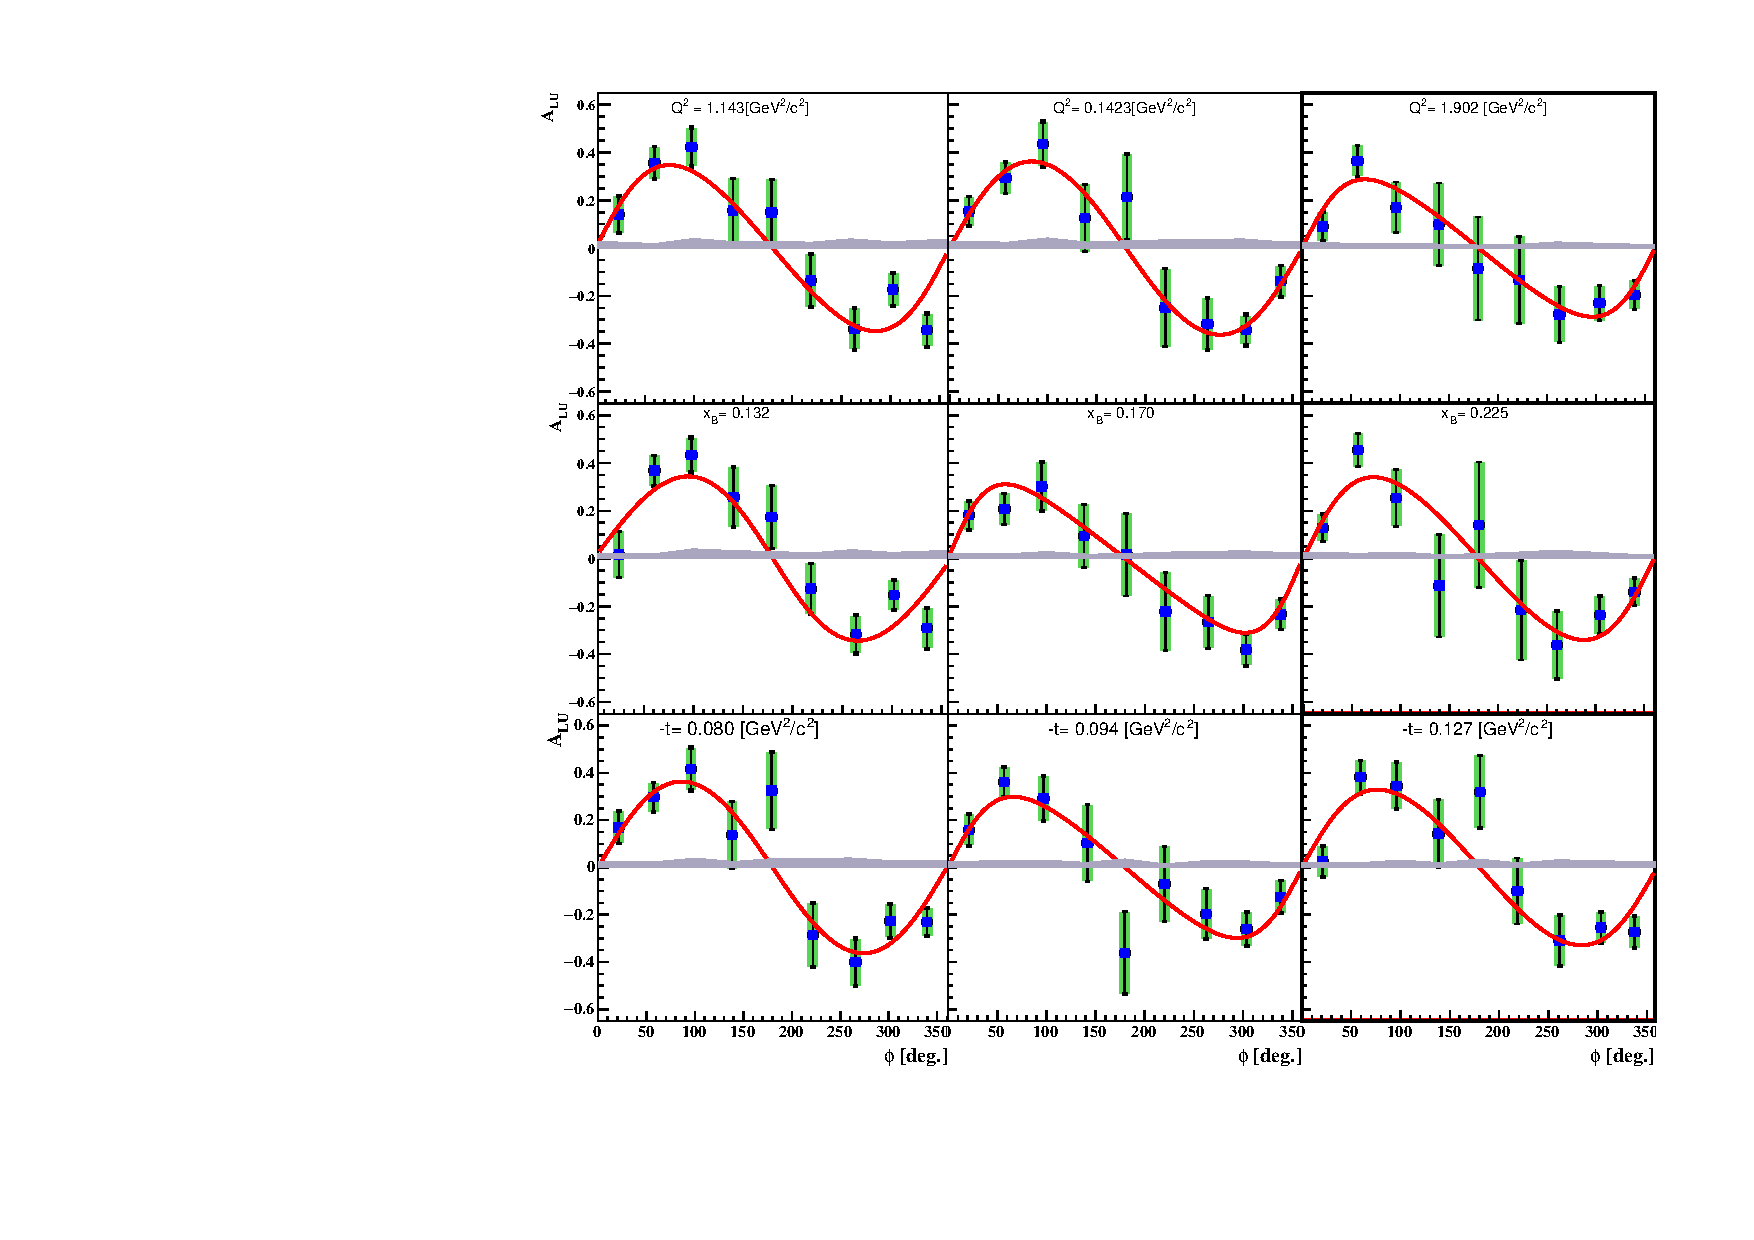
\includegraphics[height=15.0cm]{coherent-ALU.pdf}
  \caption{The reconstructed $A_{LU}$ as a function of $\phi$.}
  \label{fig:}
 \end{figure}                                                                  



\begin{figure}[tpb]
   \centering
  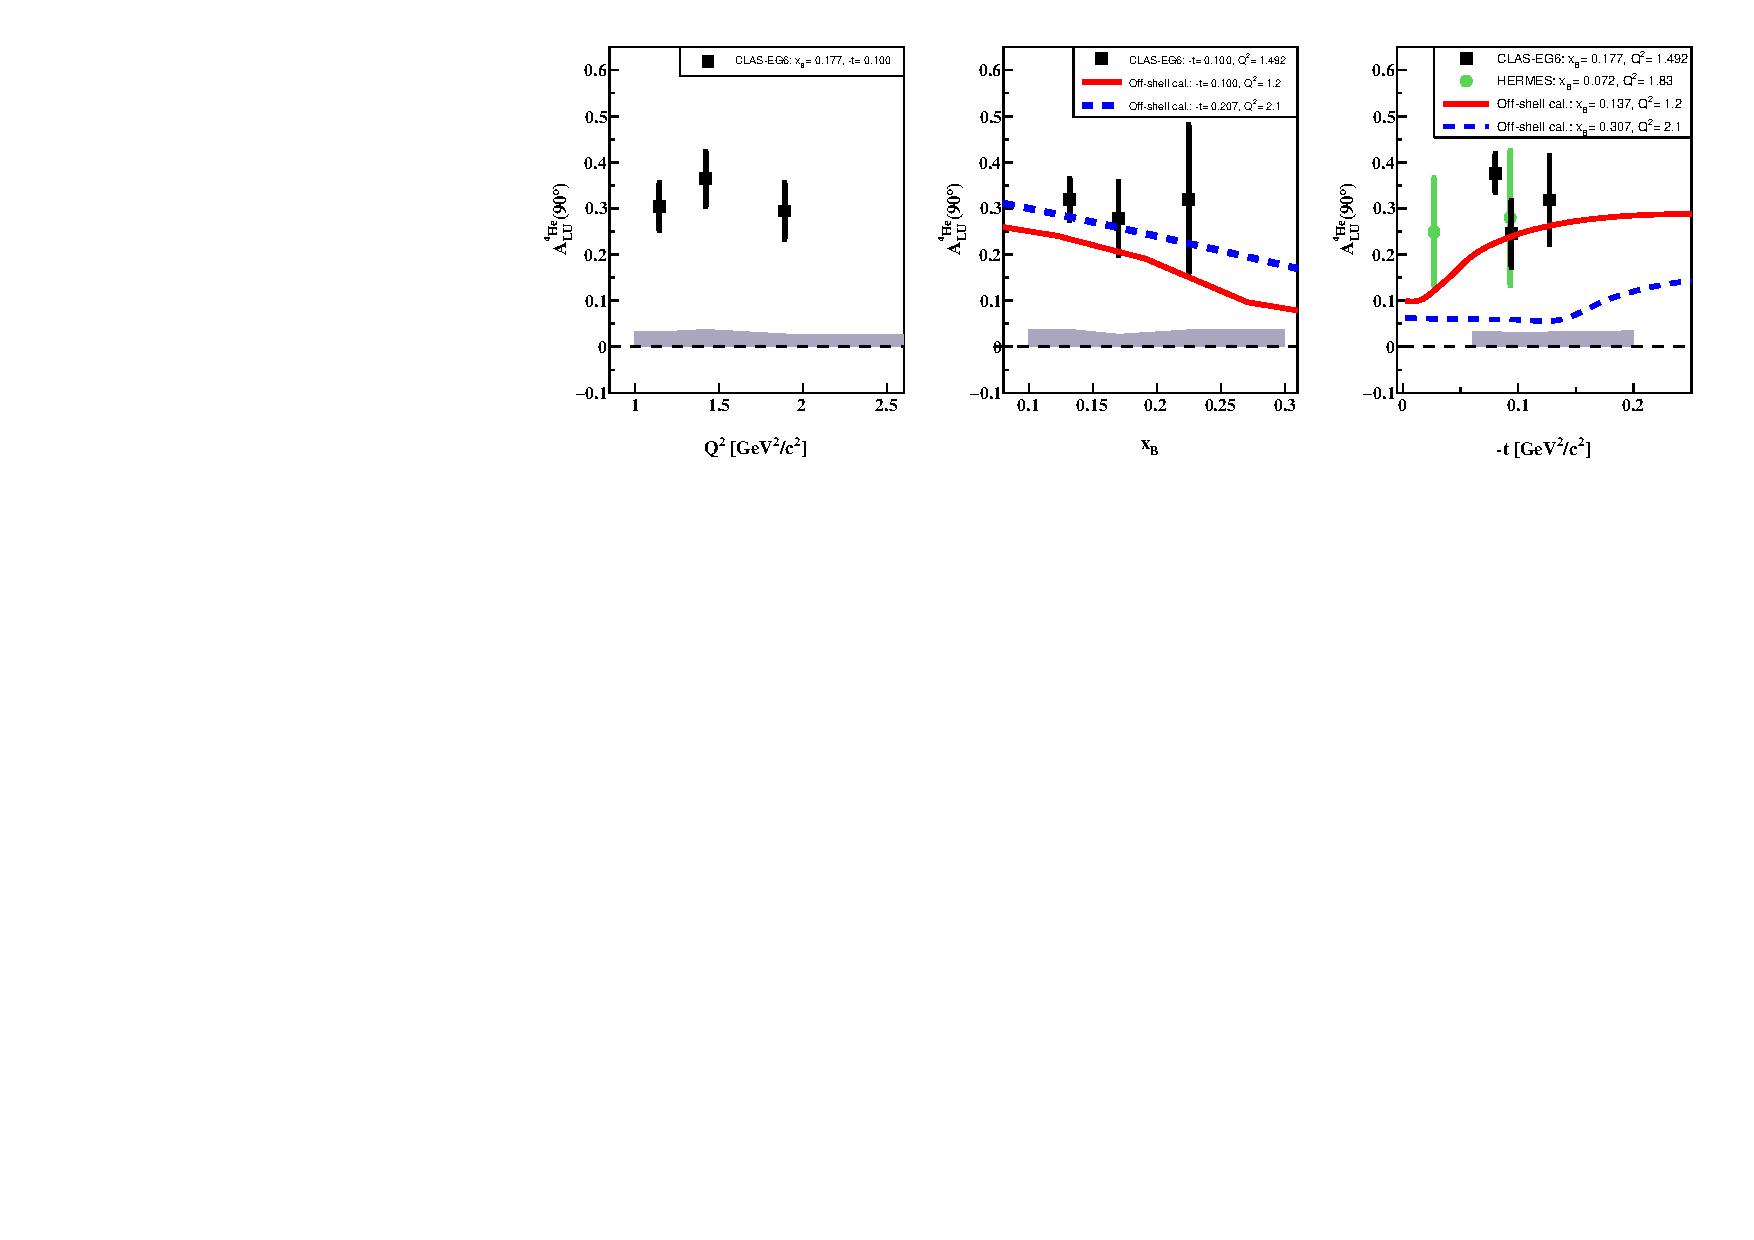
\includegraphics[height=7.0cm]{coherent-ALU_90.pdf}
  \caption{$A_{LU}$(90$^{\circ}$) vs. $Q^{2}$, $x_B$ and $-t$.}
  \label{fig:}
 \end{figure}                                                                  

\begin{figure}[tpb]
   \centering
  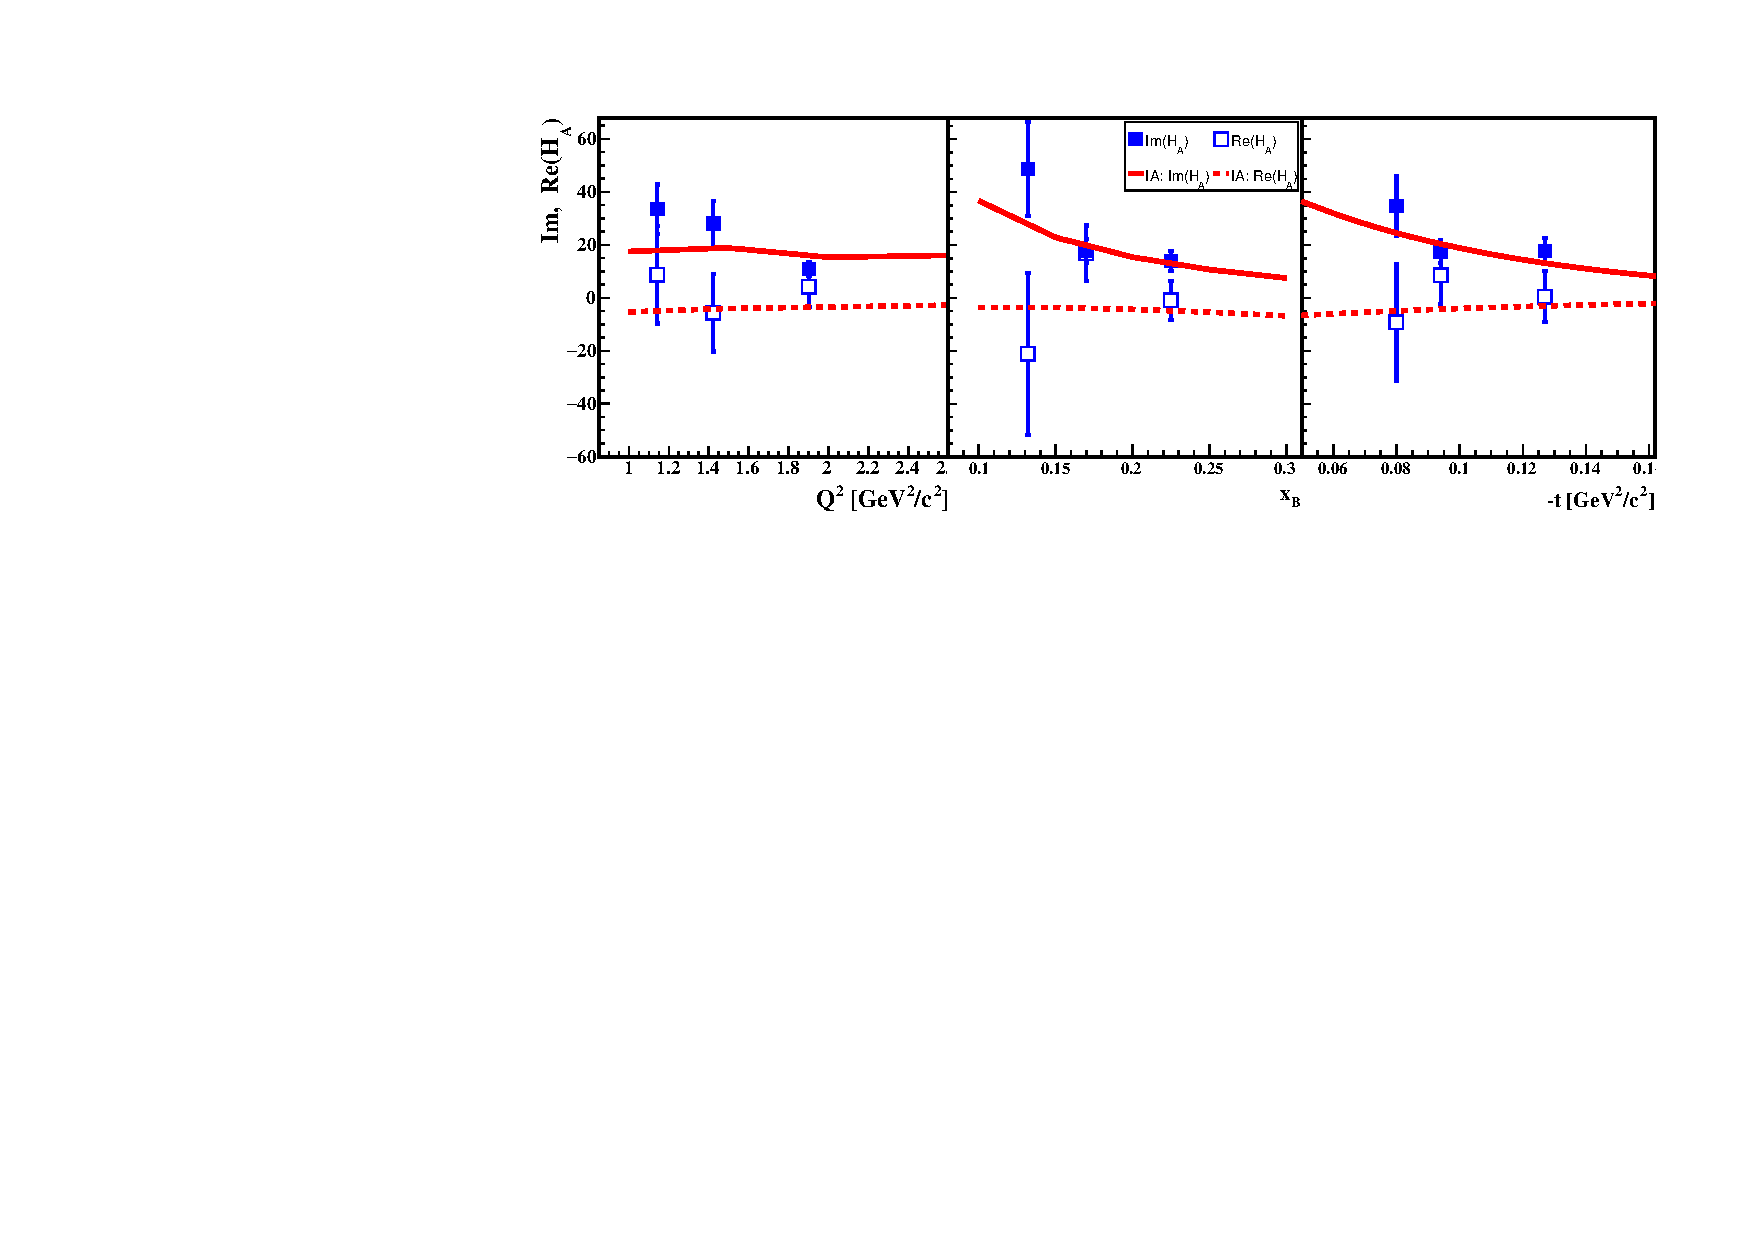
\includegraphics[height=7.0cm]{He_CFF_HA.pdf}
  \caption{The real and imaginary parts of $^4$He CFF as a function of $Q^{2}$, 
  $x_B$ and $-t$.}
  \label{fig:}
 \end{figure}                                                                  


%\bibliographystyle{abbrv}
%\bibliography{main}

\end{document}
